\subsubsection{Definición de entradas y salidas de las redes neuronales}\label{inputs-outputs}

Antes de continuar explicando los pasos llevados a cabo hay que diseñar que \textit{dataset} se necesita para entrenar a las redes neuronales. Uno de los principales requisitos en el diseño de redes neuronales es la correcta especificación del vector de entrada y salida de la red neuronal. La cantidad de variables y el tipo de variables que se usarán en la red es una de las principales claves para que el modelo funcione de forma satisfactoria. En este apartado se explicará tanto la estructura del vector de entrada como la estructura del vector de salida acompañado de ejemplos gráficos.
\newline

Los modelos con los que trabajaremos tendrán como entrada valores que representan la fecha y la hora representados con los siguientes atributos: \textit{hour} (h), \textit{day\_of\_week}(d) y \textit{month}(m). Es decir, los viajes se agruparan por intervalos, creando de este modo una nueva columna que se denominará \textit{quantity\_$j$} (q), siendo $j$, el índice de la estación. En total hay $633$ estaciones en la ciudad de Chicago. Por lo que para cada intervalo, la red neuronal contará con $636$ valores de entrada. Se pueden ver ejemplos gráficos en la Figura \ref{fig:models-design-1} y \ref{fig:models-design-2}.
\newline

Si se quiere usar más intervalos para que la red entrene, el vector resultante tendrá un número de elementos múltiplo de $636$. Por ejemplo, si se quieren usar 5 intervalos como vector de entrada, entonces la red tendrá una primera capa con $636 \times 5 = 3180$ unidades o neuronas. Por otro lado, se podrían usar más variables conteniendo información importante como puede ser el calendario laboral o variables relacionadas con la meteorología, las cuales influyen en los patrones de comportamiento de la red de bicicletas.
\newline

Por ejemplo, un lunes no laboral, la cantidad de bicicletas alquiladas en un parque será mayor que cualquier otro lunes de otra semana. U otro ejemplo, si un día las condiciones meteorológicas nos son favorables para el uso de bicicleta, la cantidad de bicicletas alquiladas se reducirán considerablemente. Este tipo de variables son algún ejemplo que se podría añadir al \textit{dataset} y así poder mejorar la precisión del modelo pero por falta de tiempo y por simplicidad no se han añadido. Además, los resultados obtenidos de por sí se han considerado bastante buenos y por lo tanto, no se ha visto la necesidad de invertir tiempo en este apartado aunque sería un buen estudio como mejoraría estos modelos con dichos cambios.
\newline

Por otra parte, la salida de la red será un vector que contenga la predicción para todas las estaciones de la red. Es decir, se calculará un vector donde cada valor será la predicción de alguna de las estaciones de la red en un intervalo en concreto. La longitud del vector por lo tanto vendrá dado por el número de estaciones con las que se trabaje, que en total son $633$ multiplicado por la cantidad de intervalos que se quieren predecir, es decir, el vector resultante tendrá $633 \times \text{n\_stations}$ valores. 
\newline

En los modelos autoregresivos, a pesar de ser modelos capaces de predecir múltiples intervalos si fuese neceario, la salida de estos modelos siempre serán de un intervalo. Esto es debido a que es necesario calcular todos los intervalos de forma independiente pues el modelo autoregresivo usa su propia predicción como vector de entrada. Se puede ver más información sobre esto en la Sección \ref{window_ar} y \ref{model_ar}.
\newline

A continuación, se pueden ver gráficamente varios ejemplos de distintas configuraciones de red usando diferentes combinaciones para la cantidad de intervalos de entrada y salida:


\begin{figure}[H]
    \centering
    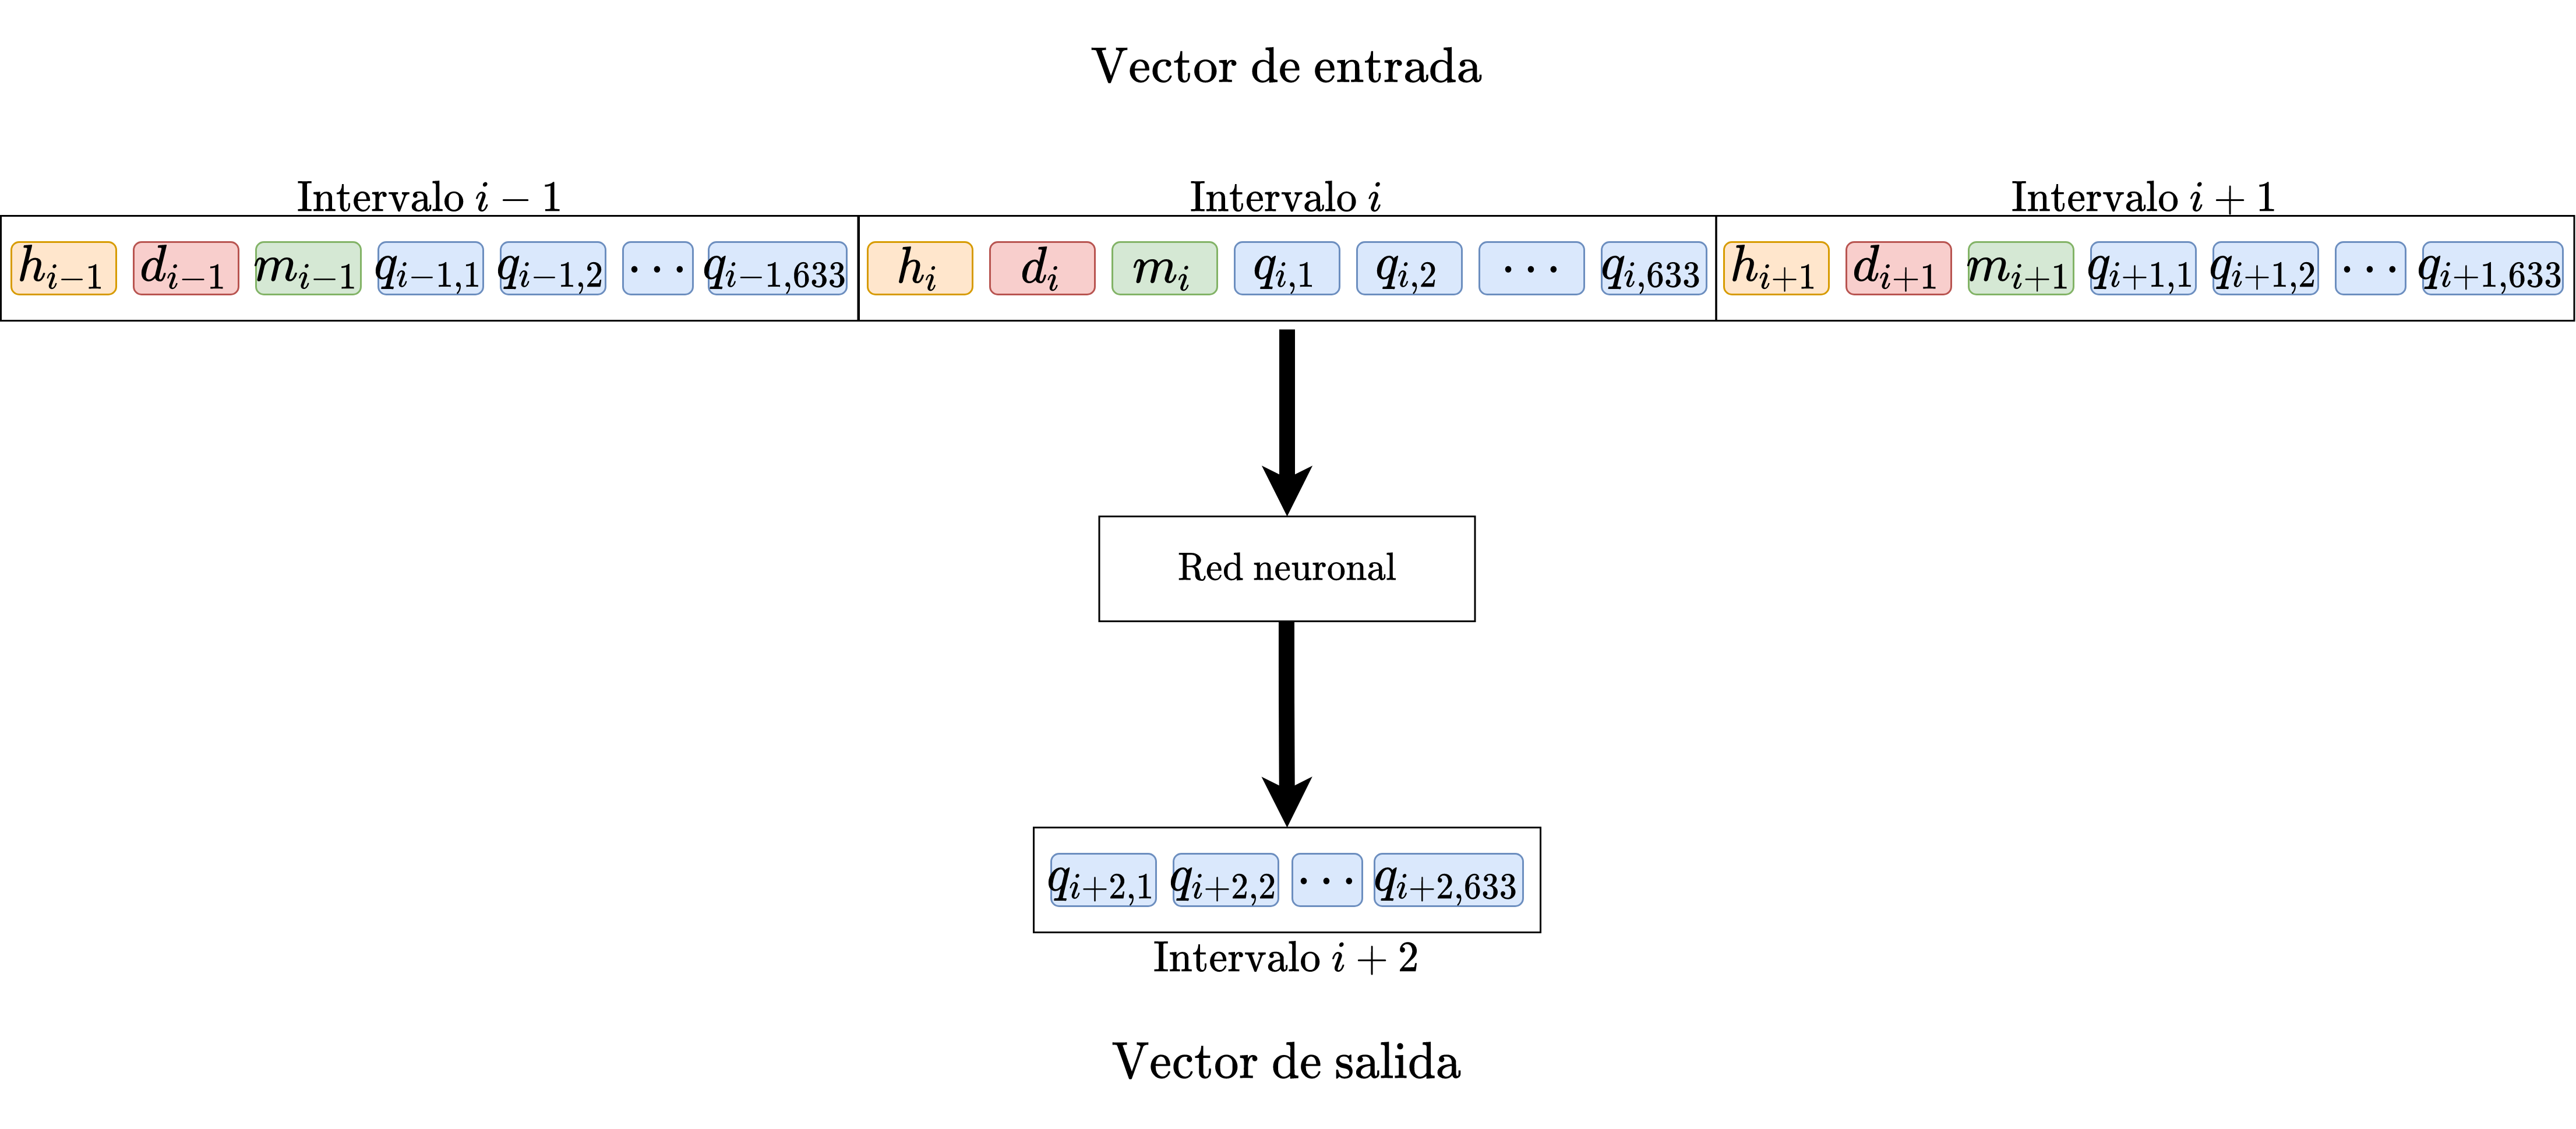
\includegraphics[width=14cm]{images/solution/preprocessing/models-design-1.png}
    \caption{Ejemplo de red neuronal que usa 3 intervalos de entrada y predice 1 intervalo}
    \label{fig:models-design-1}
\end{figure}

\begin{figure}[H]
    \centering
    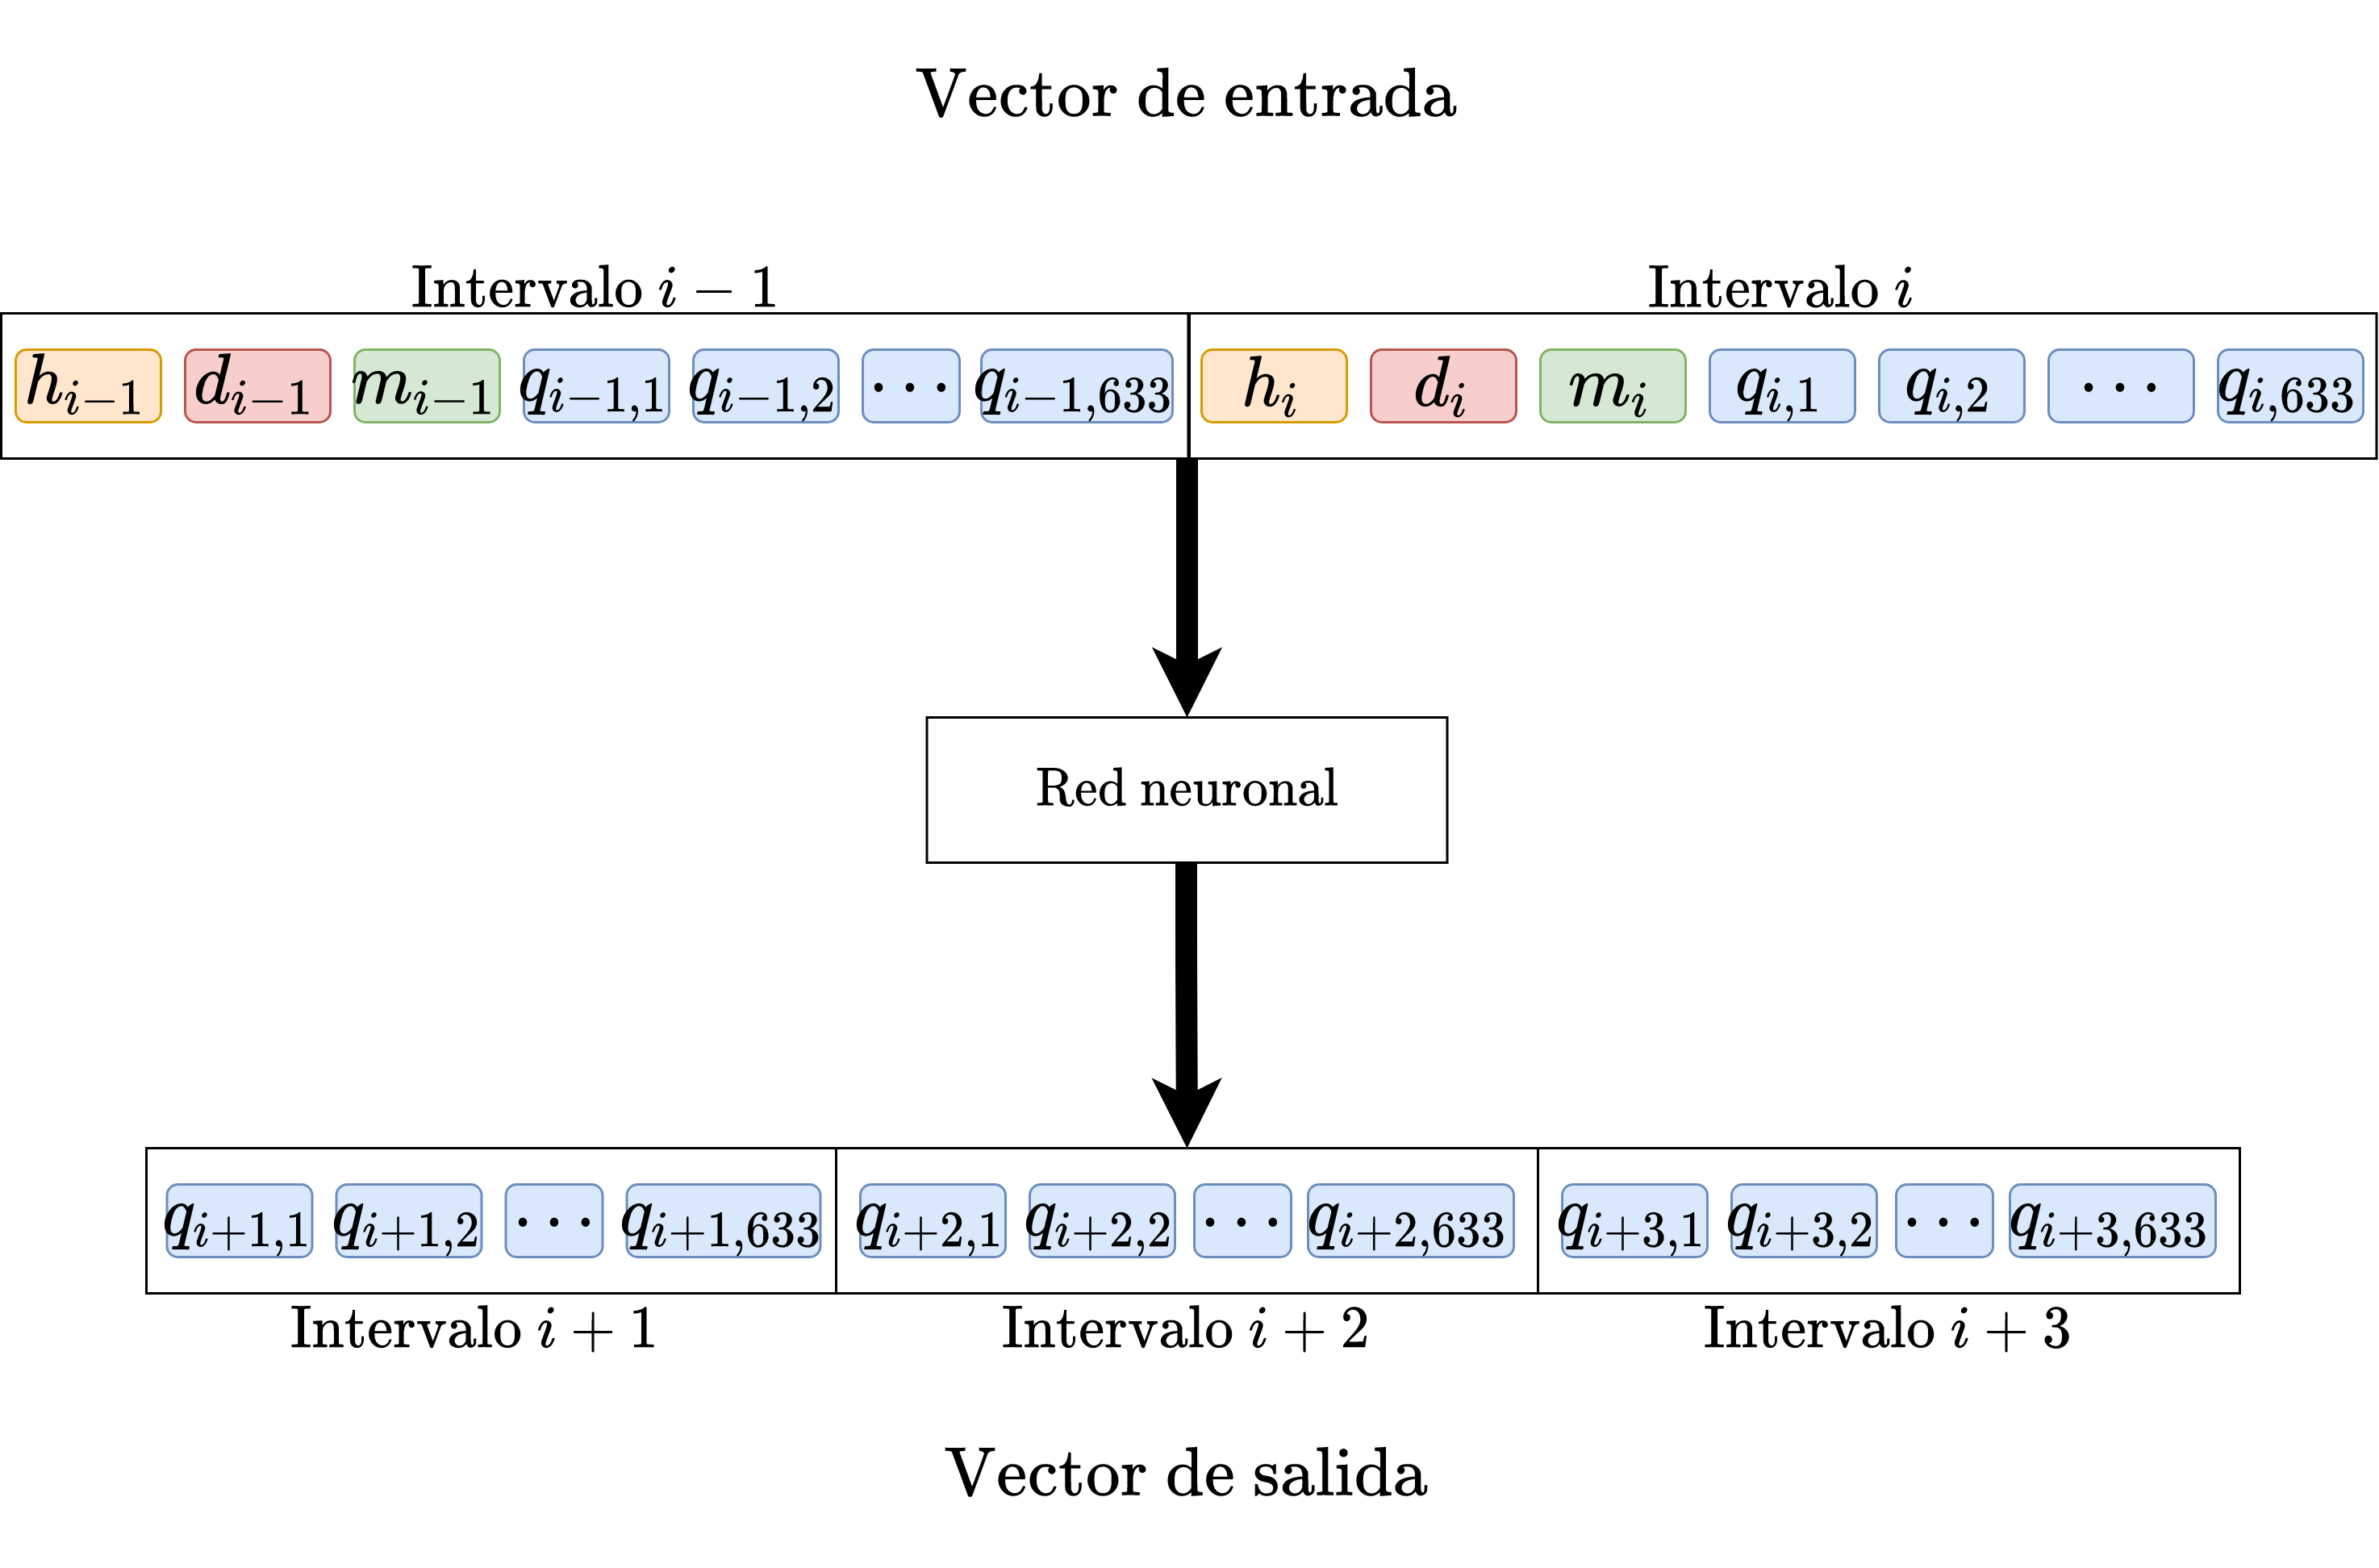
\includegraphics[width=14cm]{images/solution/preprocessing/models-design-2.png}
    \caption{Ejemplo de red neuronal que usa 2 intervalos de entrada y predice 3 intervalos}
        \label{fig:models-design-2}
\end{figure}



Esta estructura, nos permite trabajar con un número variable de estaciones siendo los modelos fácilmente exportables a otras ciudades y otras redes donde la cantidad de estaciones sea distinta. O incluso, si se quisiese trabajar con una única estación se podría realizar sin ningún problema, puesto que cada estación es representada con su propia columna. El código desarrollado para que los modelos funcionen es fácilmente reutilizable para un conjunto de estaciones más pequeñas u otras ciudades o incluso otros problemas de la misma índole, solo haría falta modificar el módulo de \textit{feature-selection} y preprocesamiento.